\documentclass[../main.tex]{subfiles}

\graphicspath{{\subfix{../images/}}}

\begin{document}

\section{Task 3.4}

Create a cycle accurate communication model of a master and slave module that uses the Avalon Streaming Bus Interface (ST). Simulate that a master are transmitting data to a slave module as illustrated in Figure (\ref{fig:avalon}). The slave should store received data from the master in a text file. Include in the model a situation where the data sink signals $\text{ready} = \text{'0'}$. The simulated result should be presented in the GTK wave viewer, so a VCD trace file must be created. It should e possible to configure the channel, error and data size define in a separate header file.

\begin{figure}[h]
    \centering
    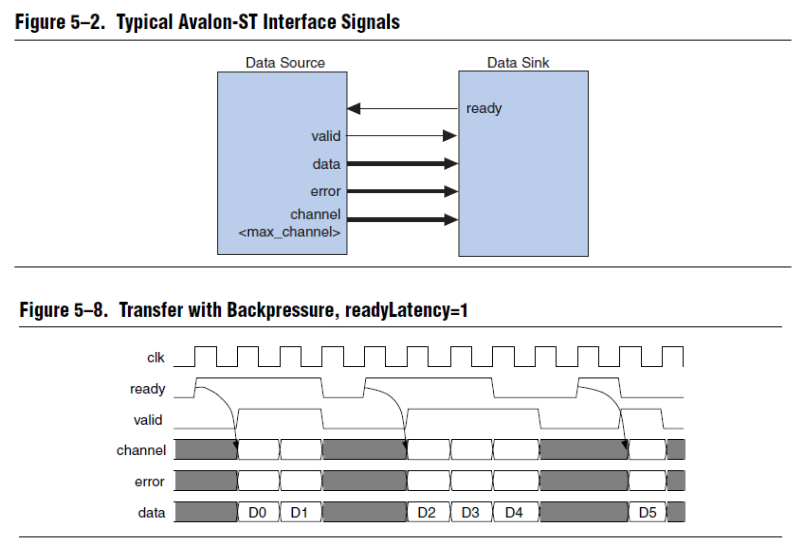
\includegraphics[width=0.85\textwidth]{task3_4.png}
    \caption{Avalon Streaming Bus Interface.}
    \label{fig:avalon}
\end{figure}

\subsection*{Solution}

We started by creating a \texttt{AvalonConf.hpp} header for containing channel defines. It also creates a typedef depending on the width of the data channel. The interface supports a data width of 8, 16, 32 and 64 bits.

\begin{myminted}{/inc/AvalonConf.hpp}
/* Avalon Channel Configuration */
#define CHANNEL_BITS    4   /* Number of channel wires      */
#define ERROR_BITS      2   /* Number of error wires        */
#define DATA_BITS       16  /* Number of data wires         */
#define MAX_CHANNEL     2   /* Maxinum number of channels   */

#if DATA_BITS == 8
typedef uint8_t binMessageType;
#elif DATA_BITS == 16
typedef uint16_t binMessageType;
#elif DATA_BITS == 32
typedef uint32_t binMessageType;
#elif DATA_BITS == 64
typedef uint64_t binMessageType;
#endif
\end{myminted}

\newpage

\begin{myminted}{/inc/AvalonMaster.hpp}
class AvalonMaster : public sc_module {
public:
    sc_in<bool>                     clk;
    sc_in<bool>                     ready;
    sc_out<bool>                    valid;
    sc_out<sc_int<DATA_BITS>>       data;
    sc_out<sc_int<CHANNEL_BITS>>    channel;
    sc_out<sc_int<ERROR_BITS>>      error;

    AvalonMaster(sc_module_name name);
    ~AvalonMaster();

private:
    std::string moduleName;
    std::string message;
    binMessageType binaryPacket;
    void transmit();
};
\end{myminted}


\end{document}